\documentclass[border=4pt]{standalone}
\usepackage{fontspec}
\usepackage{amsmath}
\usepackage{unicode-math}
\setmainfont{Latin Modern Roman}
\setmathfont{Latin Modern Math}
\usepackage{pgfplots}
\usepackage{pgfplotstable}
\pgfplotsset{compat=1.18}
\usepackage{tkz-euclide}
\usetikzlibrary{arrows.meta,calc,angles,quotes,patterns,3d,backgrounds}
\definecolor{ink}{HTML}{123428}
\definecolor{asy}{HTML}{475569}
\definecolor{mint}{HTML}{86e0bd}
\tikzset{asym/.style={asy, line width=0.9pt, dash pattern=on 5pt off 3.5pt},
         guide/.style={gray!70, line width=0.6pt, densely dotted},
         dot/.style={circle, inner sep=0pt, minimum size=5pt, draw=white, line width=0.5pt},
         odot/.style={circle, inner sep=0pt, minimum size=5.5pt, fill=white, line width=1pt},
         lab/.style={font=\footnotesize, inner sep=1.5pt, text=ink}}
\begin{document}
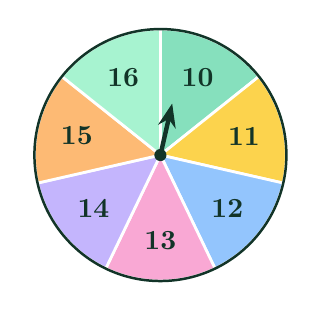
\begin{tikzpicture}
\fill[fill={rgb,255:red,134;green,224;blue,189}, draw=white, line width=1pt] (0,0) -- (90.000:1.6) arc[start angle=90.000, end angle=38.571, radius=1.6cm] -- cycle;
\node[font=\bfseries, text=ink] at (64.286:1.088) {10};
\fill[fill={rgb,255:red,252;green,211;blue,77}, draw=white, line width=1pt] (0,0) -- (38.571:1.6) arc[start angle=38.571, end angle=-12.857, radius=1.6cm] -- cycle;
\node[font=\bfseries, text=ink] at (12.857:1.088) {11};
\fill[fill={rgb,255:red,147;green,197;blue,253}, draw=white, line width=1pt] (0,0) -- (-12.857:1.6) arc[start angle=-12.857, end angle=-64.286, radius=1.6cm] -- cycle;
\node[font=\bfseries, text=ink] at (-38.571:1.088) {12};
\fill[fill={rgb,255:red,249;green,168;blue,212}, draw=white, line width=1pt] (0,0) -- (-64.286:1.6) arc[start angle=-64.286, end angle=-115.714, radius=1.6cm] -- cycle;
\node[font=\bfseries, text=ink] at (-90.000:1.088) {13};
\fill[fill={rgb,255:red,196;green,181;blue,253}, draw=white, line width=1pt] (0,0) -- (-115.714:1.6) arc[start angle=-115.714, end angle=-167.143, radius=1.6cm] -- cycle;
\node[font=\bfseries, text=ink] at (-141.429:1.088) {14};
\fill[fill={rgb,255:red,253;green,186;blue,116}, draw=white, line width=1pt] (0,0) -- (-167.143:1.6) arc[start angle=-167.143, end angle=-218.571, radius=1.6cm] -- cycle;
\node[font=\bfseries, text=ink] at (-192.857:1.088) {15};
\fill[fill={rgb,255:red,167;green,243;blue,208}, draw=white, line width=1pt] (0,0) -- (-218.571:1.6) arc[start angle=-218.571, end angle=-270.000, radius=1.6cm] -- cycle;
\node[font=\bfseries, text=ink] at (-244.286:1.088) {16};
\draw[ink, line width=0.9pt] (0,0) circle (1.6);
\draw[ink, line width=1.6pt, -{Stealth[length=3mm]}] (0,0) -- (77.143:0.672);
\fill[ink] (0,0) circle (2.2pt);
\end{tikzpicture}
\end{document}
